% Kap. 5 -- Neuaufbau 2026-11-06, Stil "luftig" (Backup: ../elektronik-1_backup_2026-11-05)
\section{Analog-Digital-Wandler (ADC)}\label{sec:adc}

\subsection{Grundbegriffe}\label{sec:adc-grund}

$$ \boxed{ q = \frac{V_{\rm refp}-V_{\rm refn}}{2^n} } \qquad
   \boxed{ D = \Big\lfloor \frac{V_{\rm in}-V_{\rm refn}}{q} \Big\rfloor } \;\;\text{(abgeschnitten)} $$
Quantisierungsfehler $|E_q| < \frac12\,$LSB nur mit Runden, sonst $0\dots 1\,$LSB. \\[2pt]

\textbf{Sample \& Hold}: hält $V_{\rm in}$ während der Wandlung fest; mit OpAmp-Buffer, sonst Belastung der Quelle. \\[2pt]
\textbf{Settling} nach vollem Sprung: \; auf 1 LSB: $t = RC\ln 2^n$, \; auf $\pm\frac12$ LSB: $t = RC\ln 2^{n+1}$

\vspace{3pt}
{\renewcommand{\arraystretch}{1.45}
\begin{tabularx}{\columnwidth}{@{}l X l l l@{}}
	\toprule
	\textbf{Prinzip}           & \textbf{Takte}                     & \textbf{Auflösung} & \textbf{Rate} & \textbf{Leistung} \\ \midrule
	Flash / Pipeline           & 1 (Pipeline: 1 Wert pro Takt)      & 8--14 Bit          & sehr hoch     & hoch \\
	SAR / Iterativ             & $n$                                & 8--20 Bit          & mittel--hoch  & mittel \\
	Integrierend / Sigma-Delta & $\gg 2^n$                          & 16--24 Bit         & niedrig       & niedrig \\ \bottomrule
\end{tabularx}}

\subsection{Flash-ADC (Parallelverfahren)}\label{sec:flash}

\begin{minipage}[c]{0.36\columnwidth}
	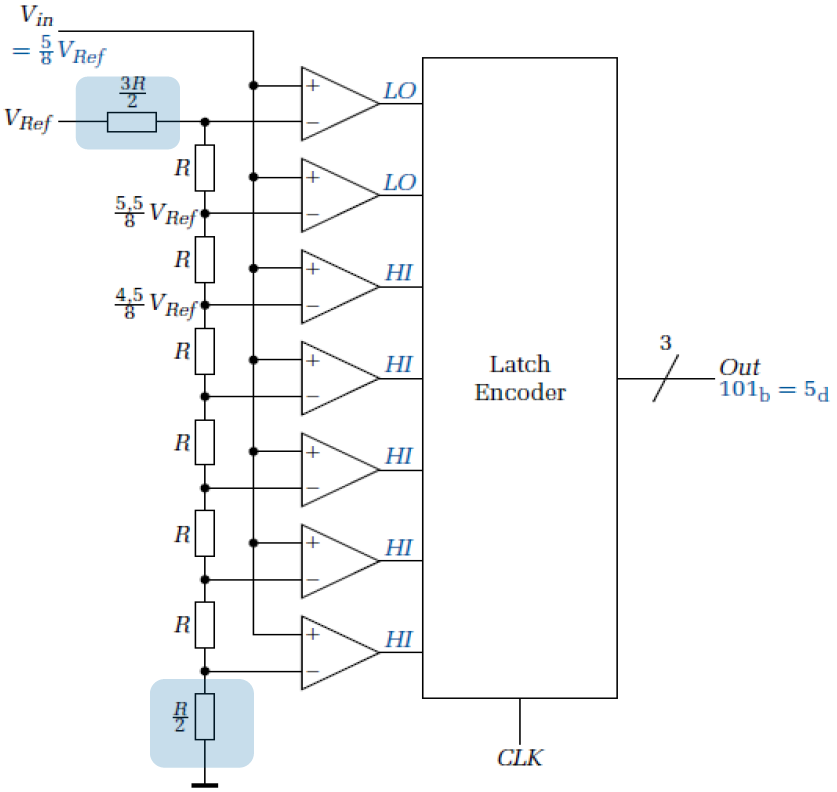
\includegraphics[width=\columnwidth]{images/ADC_parallelverfahren.png}
\end{minipage}
\hfill
\begin{minipage}[c]{0.6\columnwidth}
	$2^n$ Widerstände, \; $2^n-1$ Komparatoren, \; 1 Takt \\[4pt]
	{\renewcommand{\arraystretch}{1.5}
	\begin{tabular}{@{}l l l@{}}
		\toprule
		                & \textbf{Alle $R$ gleich}  & \textbf{unten $\frac R2$, oben $\frac{3R}{2}$} \\ \midrule
		Schwelle $i$    & $i\cdot q$                & $\big(i-\frac12\big)\,q$ \\
		Code            & ${\rm floor}(V_{\rm in}/q)$ & ${\rm round}(V_{\rm in}/q)$ \\
		Kaskade         & möglich                   & nicht möglich \\ \bottomrule
	\end{tabular}}
\end{minipage}

\vspace{3pt}
\textbf{Code} = Anzahl Schwellen unter $V_{\rm in}$ (bleibt bei $2^n-1$ stehen).

\warn{\textit{«b[3:1] = 1» significa codice 1, non 111.}}

\subsection{Pipeline und iterativer ADC: binäre Suche}\label{sec:pipeline}

\begin{minipage}[c]{0.44\columnwidth}
	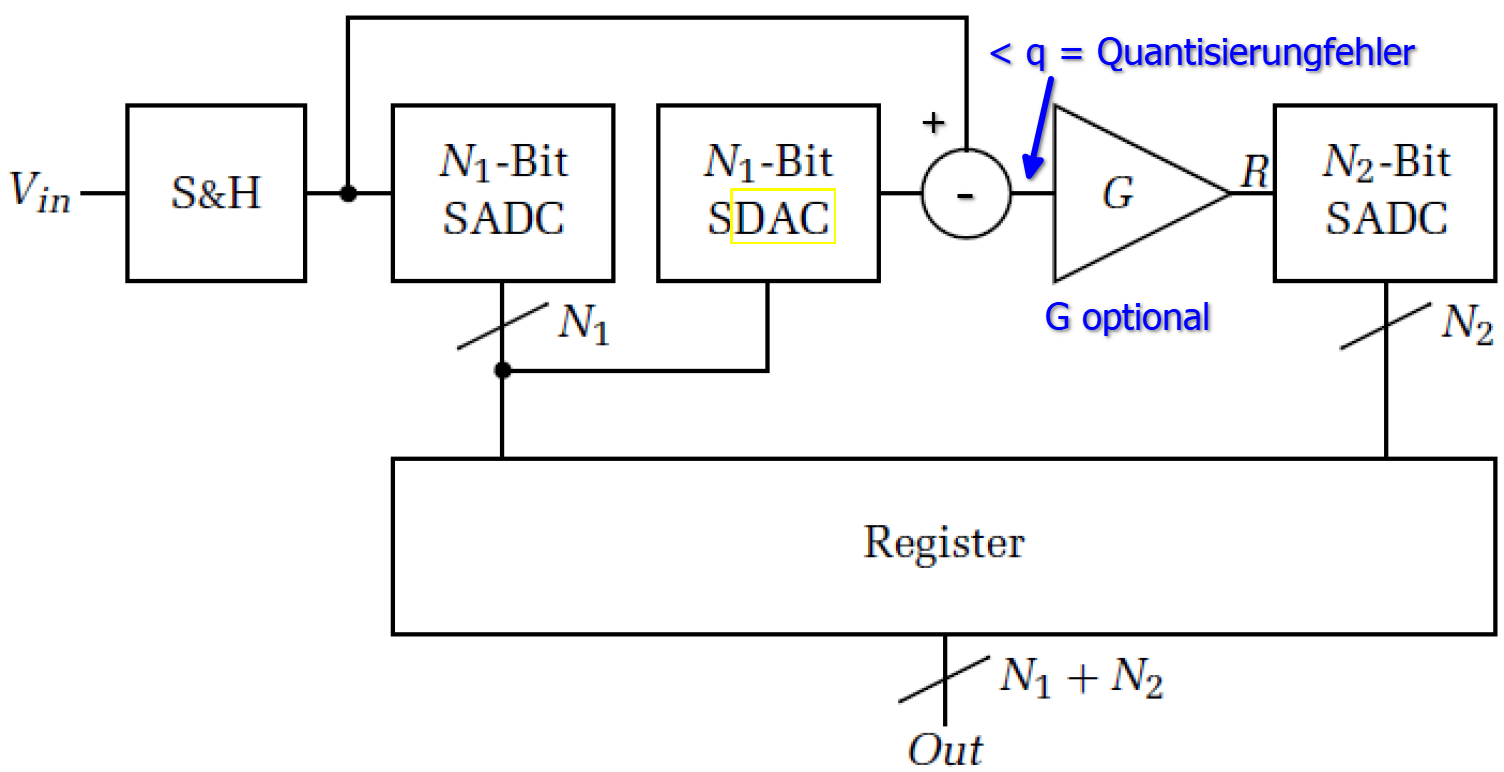
\includegraphics[width=\columnwidth]{images/pipeline_ADC.png}
\end{minipage}
\hfill
\begin{minipage}[c]{0.52\columnwidth}
	\textbf{Subranging} (2 Stufen, $N_1 + N_2$ Bits):
	$$ R = V_{\rm in} - D_1 q_1 \in [0,\,q_1) $$
	$$ V_{\rm REF2} = q_1 \;\;\text{oder}\;\; G = 2^{N_1} $$
	$$ q = \frac{V_{\rm REF}}{2^{N_1+N_2}} $$
	nur $2^{N_1}+2^{N_2}$ Komparatoren
\end{minipage}

\vspace{4pt}
{\renewcommand{\arraystretch}{1.8}
\begin{tabularx}{\columnwidth}{@{}l l X >{\raggedright\arraybackslash}p{0.14\columnwidth}@{}}
	\toprule
	\textbf{Variante}     & \textbf{Vergleich}                                 & \textbf{Rest}                                                         & \textbf{Zeit} \\ \midrule
	Pipeline 1 Bit/Stufe  & Schwelle $\dfrac{V_{\rm REF}}{2^k}$ (halbiert)      & $E_k = E_{k-1} - B_k\,\dfrac{V_{\rm REF}}{2^k}$                       & Latenz $n$, \newline 1 Wert/Takt \\
	Iterativ              & Schwelle immer $\dfrac{V_{\rm REF}}{2}$             & $V_x \leftarrow 2\Big(V_x - B\,\dfrac{V_{\rm REF}}{2}\Big)$           & $n$ Takte \\ \bottomrule
\end{tabularx}}

\begin{warnbox}
	\small
	\warn{\textit{Ogni bit a 1 \textbf{aggiunge} il suo peso; a dimezzarsi da uno stadio all'altro è il peso, non la tensione.}}
	\warn{\textit{G sbagliato \textrightarrow\ missing codes; nell'iterativo l'errore si moltiplica a ogni giro.}}
\end{warnbox}

\subsection{SAR mit Kondensator-DAC (Wägeverfahren)}\label{sec:sar}

\begin{minipage}[c]{0.42\columnwidth}
	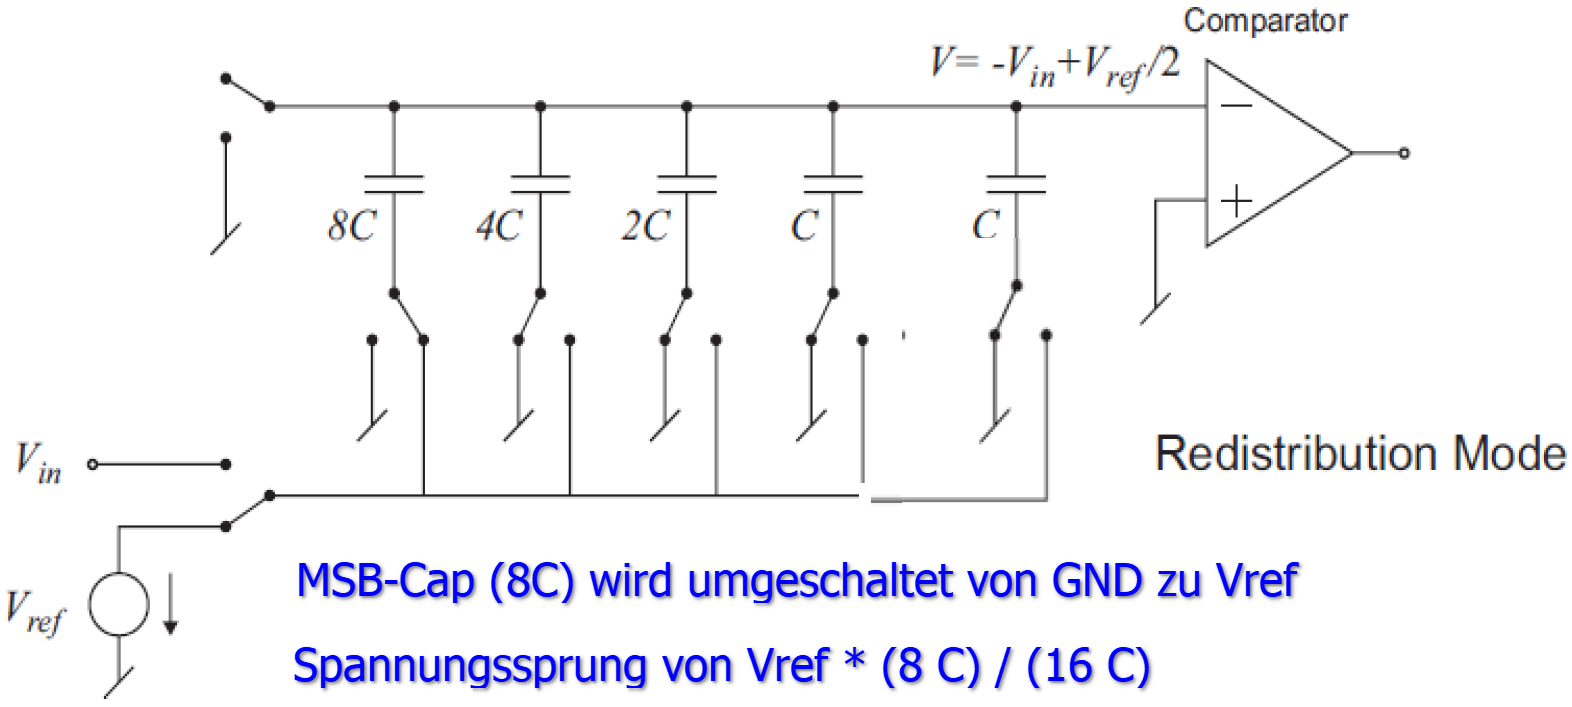
\includegraphics[width=\columnwidth]{images/SAR_switched_capacitor_redistribution_mode.png}
\end{minipage}
\hfill
\begin{minipage}[c]{0.54\columnwidth}
	\textbf{Standardfall} (Sample: obere Platte an GND):
	$$ \boxed{ V_X = -V_{\rm in} + V_{\rm ref}\,\frac{C_{\rm oben}}{C_{\rm tot}} } $$
	$C_{\rm oben}$ = \textbf{alle} $C$, die jetzt an $V_{\rm ref}$ liegen
\end{minipage}

\begin{rezept}{Rezept: SAR (jede Variante)}
	\begin{steps}
		\item \textbf{Sample}: Ladung der Insel $Q = \sum_i C_i\,(V_X - V_{u,i})$ \; ($V_{u,i}$ = untere Platte); danach konstant
		\item \textbf{Jeder Schritt}:
		      \; $V_X = \dfrac{Q + \sum_i C_i\, V_{u,i}}{C_{\rm tot}}$
		\item $V_X < 0$: Bit $=1$, Schalter bleibt auf $V_{\rm ref}$; \; $V_X > 0$: Bit $=0$, Schalter zurück auf GND
		\item Nächsten Kondensator umschalten; nach $n$ Schritten fertig
	\end{steps}
\end{rezept}

\begin{warnbox}
	\small
	\warn{\textit{In $C_{\rm oben}$ vanno \textbf{tutti} i C su $V_{\rm ref}$, non solo quello appena commutato.}}
	\warn{\textit{Bit $=0$: l'interruttore torna su GND e $V_X$ torna al valore di prima.}}
\end{warnbox}
\textbf{Kopplungs-$C$} ($\frac{32}{31}C$ in Serie): kleinere Grössenverhältnisse der Kapazitäten.

\subsection{Integrierende Wandler (Zählverfahren)}\label{sec:integrierend}

{\renewcommand{\arraystretch}{1.8}
\begin{tabularx}{\columnwidth}{@{}l l X@{}}
	\toprule
	\textbf{Wandler}  & \textbf{Formel} & \textbf{Merkmal} \\ \midrule
	Zähl (DAC-Rampe)  & Zählerstand = Code
	                  & aufgerundet, bis $2^n$ Takte \\
	Single-Slope      & $T_{\rm int} = -\dfrac{V_{\rm ref}\,RC}{V_{\rm in}}$
	                  & Zeit hängt vom Signal ab, Division nötig \\
	Dual-Slope        & $\dfrac{V_{\rm in}-V_{\rm AGND}}{V_{\rm ref}-V_{\rm AGND}} = -\dfrac{T_{\rm abint}}{T_{\rm int}} = -\dfrac{n}{N}$
	                  & $RC$ kürzt sich weg \\
	Charge Balancing  & Portion $Q = \dfrac{T_{\rm clk}\,V_{\rm ref}}{R_i}$, \; gleiche Formel $\dfrac nN$
	                  & integriert immer; grosses $N$: genau, aber langsam \\ \bottomrule
\end{tabularx}}

\vspace{3pt}
\begin{minipage}[c]{0.4\columnwidth}
	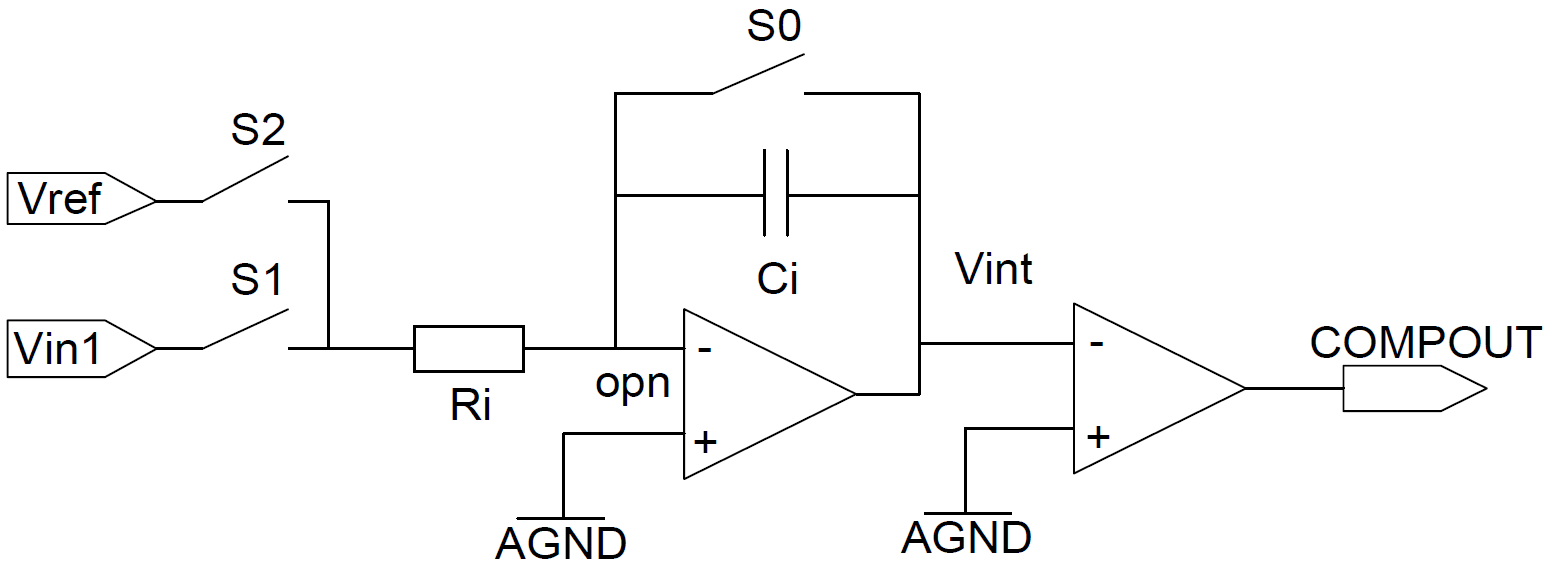
\includegraphics[width=\columnwidth]{images/dual_slope_ADC.png}
\end{minipage}
\hfill
\begin{minipage}[c]{0.24\columnwidth}
	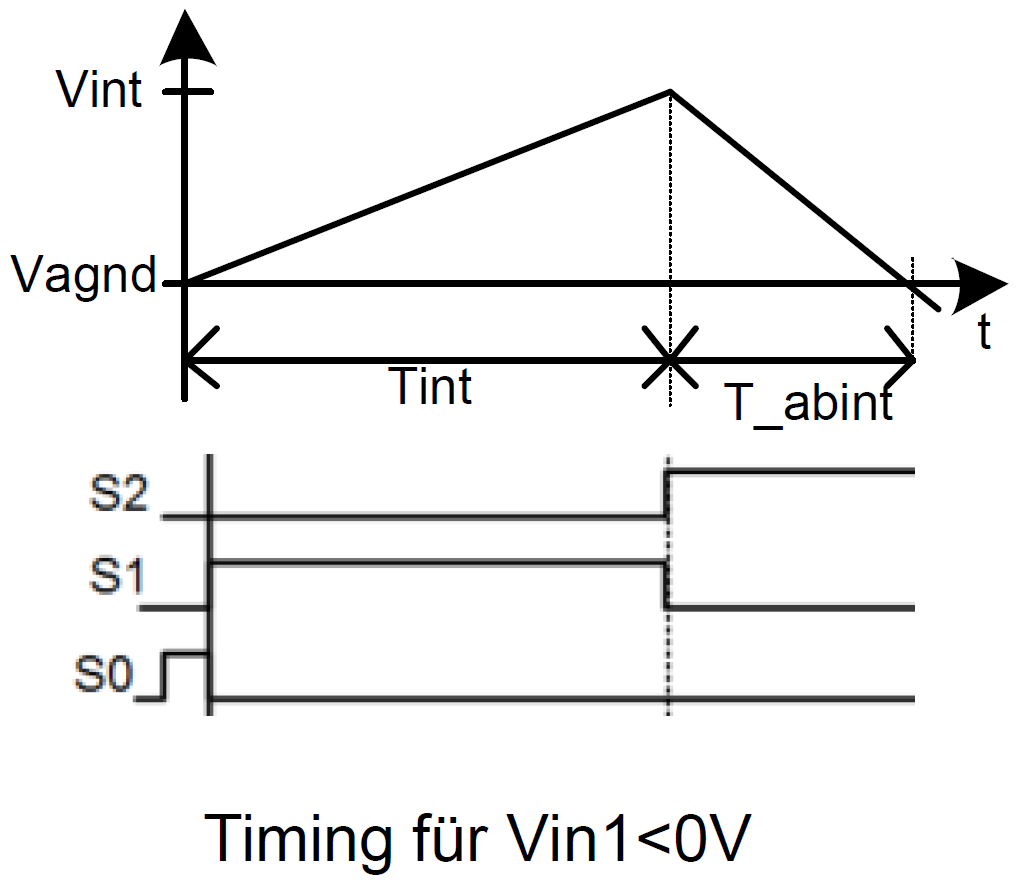
\includegraphics[width=\columnwidth]{images/dual_slope_ADC_timing.png}
\end{minipage}
\hfill
\begin{minipage}[c]{0.3\columnwidth}
	Netzbrumm: \\ $T_{\rm int} = 20\,$ms unterdrückt $50\,$Hz und Harmonische
\end{minipage}

\begin{rezept}{Rezept: Dual-Slope}
	\begin{steps}
		\item \textbf{Aufintegration} während $T_{\rm int}$:
		      \; $V_{\rm int} = V_{\rm AGND} - \dfrac{V_{\rm in}-V_{\rm AGND}}{R_iC_i}\,T_{\rm int}$
		\item \textbf{Abintegration} mit $V_{\rm ref}$ bis $V_{\rm AGND}$:
		      \; $T_{\rm abint} = T_{\rm int}\,\dfrac{V_{\rm AGND}-V_{\rm in}}{V_{\rm ref}-V_{\rm AGND}}$
		\item \textbf{Auflösung}:
		      \; $\Delta V_{\rm in} = |V_{\rm ref}-V_{\rm AGND}|\,\dfrac{T_{\rm clk}}{T_{\rm int}}$
	\end{steps}
\end{rezept}

\subsection{Fehler und Abtastung}\label{sec:adc-fehler}

{\renewcommand{\arraystretch}{1.8}
\begin{tabularx}{\columnwidth}{@{}l X@{}}
	\toprule
	\textbf{Grösse}                 & \textbf{Formel / Bedeutung} \\ \midrule
	Offset, Gain, INL, DNL          & wie beim DAC (\ref{sec:dac-fehler}) \\
	DNL durch Komparator-Offset     & $|{\rm DNL}|_{\max} = \dfrac{2V_{\rm os}}{q}$; \;
	                                  ${\rm DNL} < 1\,{\rm LSB} \Rightarrow \Delta V_{\rm REF} > 2^{n+1}\,V_{\rm os}$ \\
	Aperturfehler (Sinus, voll)     & $T_A < \dfrac{1}{2\pi f\,2^n}$ \\
	Abtasttheorem                   & $f_s > 2 f_{\max}$, sonst Aliasing \\
	Sample-Hold                     & sinc-Tiefpass: dämpft alle $f > 0$ \\
	SNR                             & $P_Q = \dfrac{q^2}{12}$, \; ${\rm SNR} = 6.02\,n + 1.76\,$dB, \;
	                                  ${\rm ENOB} = \dfrac{{\rm SNR}-1.76}{6.02}$ \\ \bottomrule
\end{tabularx}}

\warn{\textit{In $2^{n+1}V_{\rm os}$ il 2 di $2V_{\rm os}$ è già contato: non raddoppiare.}}
